\documentclass[/home/jesse/Analysis/FemtoAnalysis/AnalysisNotes/AnalysisNoteJBuxton.tex]{subfiles}
\begin{document}

\subsection{Results: \texorpdfstring{$\Xi$K$^{\pm}$}{TEXT}}
\label{ResultsXiK}

The motivation for studying the $\Xi^{-}$\Kpm system was to investigate the striking difference in the \LamKchP and \LamKchM correlation functions, as shown explicitly in Fig. \ref{fig:cLamcKchCfs0010_copy} (originally presented in Sec. \ref{TypicalCfConstruction}, and reproduced here for convenience).
The underlying cause responsible for this interesting effect is still not completely understood.
Within the femtoscopy framework presented in Section \ref{4_Femtoscopy}, it is clear that there are two important components affecting the femtoscopic signal: the pair emission source distribution, and the interaction between the particles in the pairs of interest.
We expect the pair source distribution for \LamKchP pairs to be similar to that of \LamKchM pairs, therefore, the difference in the femtoscopic signals must be due to a difference in their interactions.

\begin{figure}[h]
  \centering
  \includegraphics[width=\textwidth]{/home/jesse/Analysis/FemtoAnalysis/AnalysisNotes/4_CorrelationFunctions/Figures/canLamKchPvsLamKchM0010.pdf}
  \caption[Correlation functions: \LamKchP vs \LamKchM in 0-10\% centrality bin]{Correlation Functions: \LamKchP vs \LamKchM (\ALamKchP vs \ALamKchM) for 0-10\% centrality.  The peak in \LamKchMALamKchP at \kstar $\approx$ 0.2 GeV/c is due to the $\Omega^{-}$ (and likely the $\Xi$(1690) resonance, although to a much smaller extent).  The lines represent the statistical errors, while boxes represent systematic errors.}
  \label{fig:cLamcKchCfs0010_copy}
\end{figure}


Obviously, we do understand that the observed difference in the femtoscopic signals is due to a difference in the strong interaction in \LamKchP pairs compared to that in \LamKchM pairs; our extracted scattering parameters demonstrate that.
The interesting question to ask is, why does the strong interaction differ so significantly between the two?
The result could suggest an effect arising from different quark-antiquark interactions between the pairs, i.e. $s\bar{s}$ for \LamKchP and $u\bar{u}$ in \LamKchM.
This effect could also result from the difference in net strangeness for each system, S=0 for \LamKchP and S=-2 for \LamKchM.
It is possible that a system with less strangeness has more available channels into which it can decay, causing a scarcity of pairs, i.e. a greater suppression, of the correlation function at low \kstar.
However, such an effect should manifest itself in the imaginary component of the scattering length, $\Im f_{0}$, not the real component, $\Re f_{0}$.

In any case, to help find an explanation for this result, it would be useful to study another system where we might anticipate similar effects to be exhibited.
The $\Xi^{0}$\Kpm system is an ideal candidate, as the quark content of the $\Xi^{0}$ is \textit{uss}.
Therefore, studying $\Xi^{0}$\Kpm correlations would allow for the investigation of the $s\bar{s}$ vs. $u\bar{u}$ quark-antiquark picture.
However, the $\Xi^{0}$ unfortunately decays as $\Xi^{0} \rightarrow \Lambda \pi^{0}$, and neutral pions are difficult to detect.
The next best option is the $\Xi^{-}$\Kpm system, as the $\Xi^{-}$ has quark content \textit{dss}.
In this case, we are not able to explore the $s\bar{s}$ vs. $u\bar{u}$ picture, but we are able to investigate $s\bar{s}$ vs. the absence of any $q\bar{q}$ interaction.
Furthermore, although the net strangeness in the systems here are different than those in the \LamKpm systems (S=-1,-3 instead of S=0), studying $\Xi^{-}$\Kpm does allow us to explore the effect of different net strangeness in similar systems.
So, in comparing the $\Xi^{-}$\Kpm and \LamKpm systems, $\Xi^{-}$\KchP (S=-1, $s\bar{s}$ picture) is analogous to \LamKchP (S=0, $s\bar{s}$ picture), and $\Xi^{-}$\KchP (S=-3, absence of $q\bar{q}$ picture) is analogous to \LamKchM (S=-2, $u\bar{u}$ picture).

Figure \ref{fig:XiKchwConjResults} presents experimental data from our femtoscopic analysis of $\Xi^{-}$\Kpm pairs, along with the conjugate systems.
Even without any fits to the data, the fact that the $\Xi^{-}$K$^{+}$ data dips below unity (Fig. \ref{fig:XiKchwConjResults}) is exciting, as this cannot occur purely from a Coulomb interaction.  
We hope that this dip signifies that we are able to peer through the overwhelming contribution from the Coulomb interaction to see the effects arising from the strong interaction.

\begin{figure}[h]
  \centering
  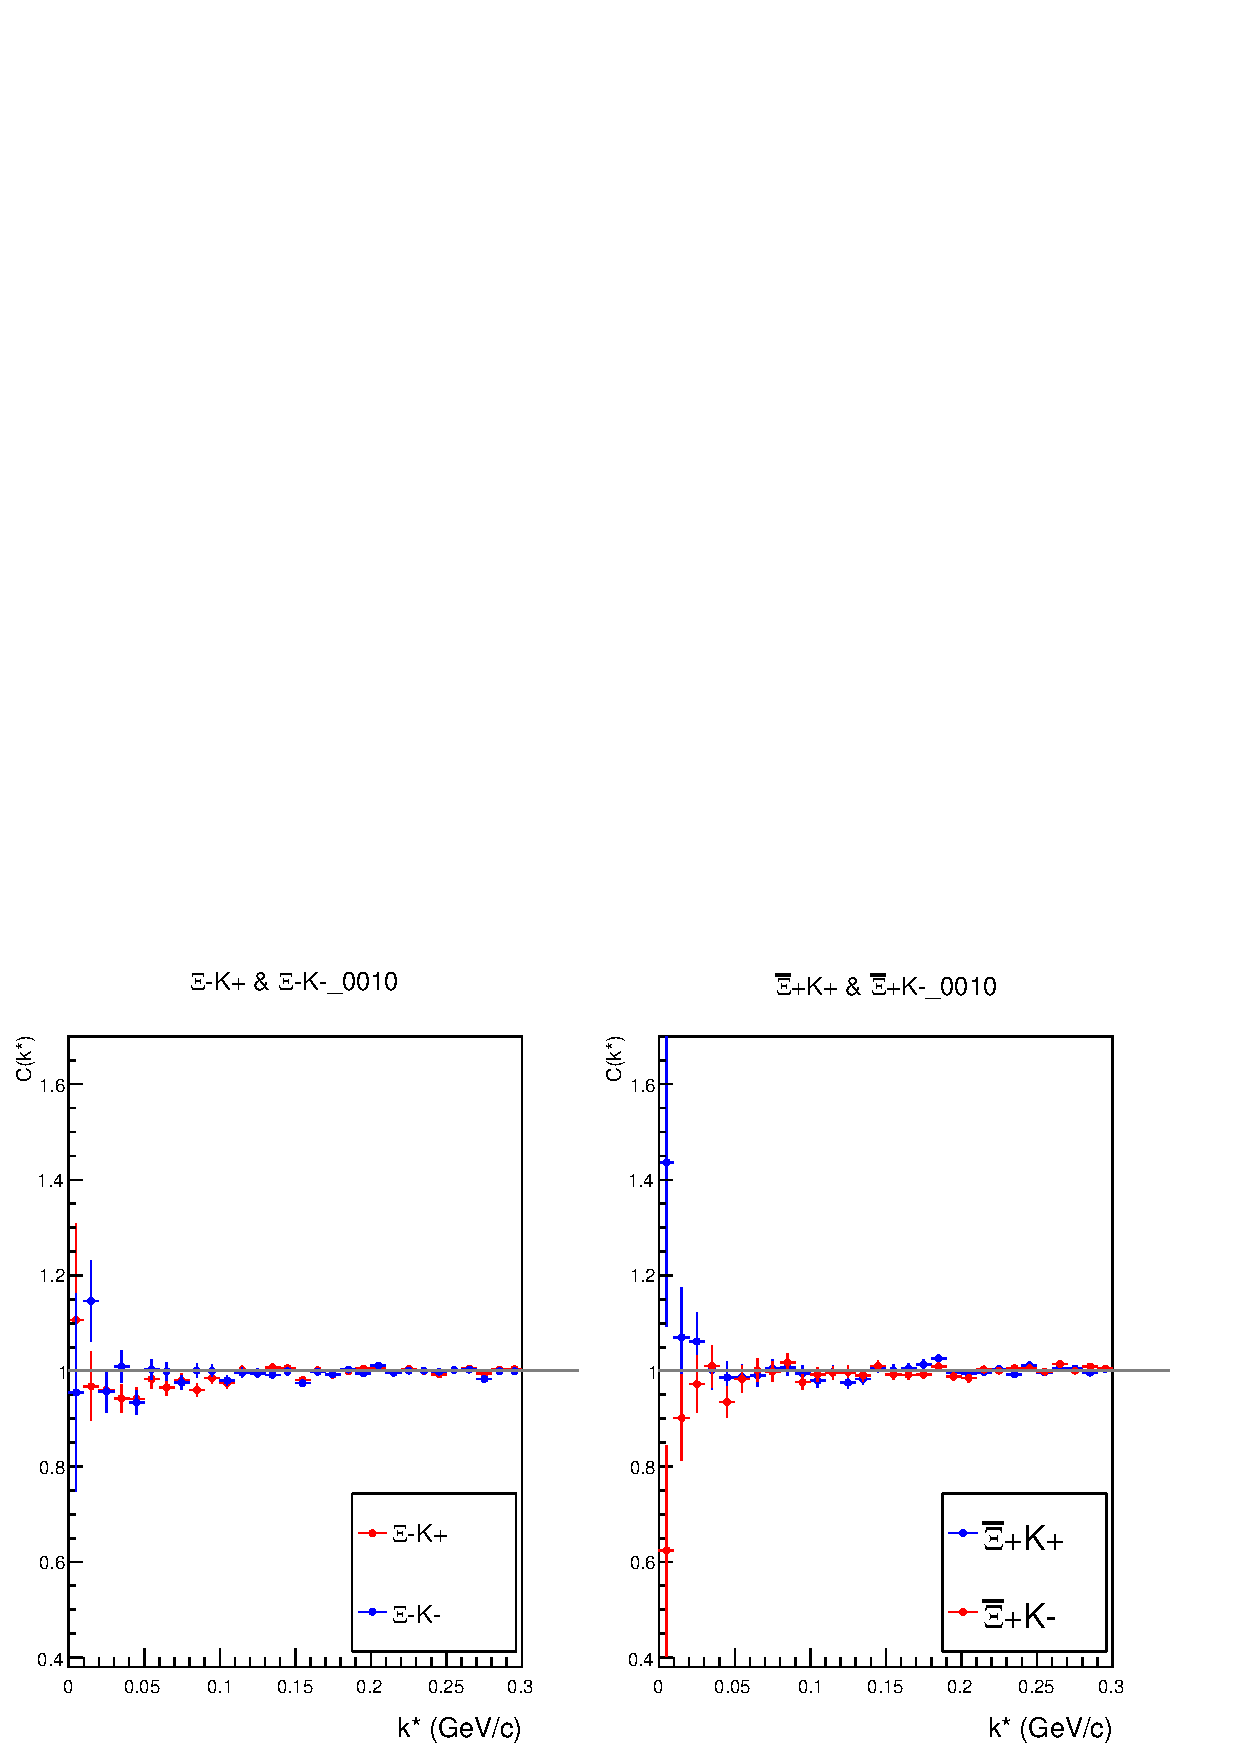
\includegraphics[width=\textwidth]{/home/jesse/Analysis/FemtoAnalysis/AnalysisNotes/7_ResultsAndDiscussion/Figures/cXicKchKStarCfs.png}
  \caption[$\Xi$K$^{\pm}$ results]{$\Xi$K$^{\pm}$ Results for 0-10\% Centrality.  (Left) $\Xi^{-}$K$^{+}$ and  $\Xi^{-}$K$^{-}$  (Right) $\bar{\Xi}^{+}$K$^{+}$ and  $\bar{\Xi}^{+}$K$^{-}$}
  \label{fig:XiKchwConjResults}
\end{figure}

%%%%%%%%%%%%%%%%%%%%%%%%%%%%%%%%%%%%%%%%%%%%%%%%%%%%%%%%%%%%%%%%%%%%%%%%%%%%%%%%%%%%%%%%
\begin{comment}
\begin{figure}[h!]
  \centering
  %%----start of first subfigure---  
  \subfloat[$\Xi$K$^{+}$ First Fit, 0-10\% Centrality]{
    \label{fig:XiKchFits:a}
    \includegraphics[width=0.49\textwidth]{7_ResultsAndDiscussion/Figures/XiKchP.pdf}}
  %%----start of second subfigure---
  \subfloat[$\bar{\Xi}$K$^{+}$ First Fit, 0-10\% Centrality]{
    \label{fig:XiKchFits:b}
    \includegraphics[width=0.49\textwidth]{7_ResultsAndDiscussion/Figures/AXiKchP.pdf}}
  %%----overall caption----
  \caption[$\Xi$K$^{\pm}$ First Fits]{$\Xi$K$^{\pm}$ First Fits}
  \label{fig:XiKchFits}
\end{figure}
\end{comment}
%%%%%%%%%%%%%%%%%%%%%%%%%%%%%%%%%%%%%%%%%%%%%%%%%%%%%%%%%%%%%%%%%%%%%%%%%%%%%%%%%%%%%%%%

Figure \ref{fig:XiKchCoulombOnlyBand} demonstrates that the $\Xi^{-}$K$^{+}$ results cannot be described by solely the Coulomb interaction.  
In this figure, we present the data along with a Coulomb-only band.  The Coulomb-only band is spanned by two Coulomb-only curves, whose parameters are given in the figure. 
The Coulomb-only curves were generated using a technique identical to the generation of the fit function, described in Sec. \ref{ModelCascadeKaon}, except, of course, with the nuclear scattering parameters all set to zero.  
The Coulomb-only curves change monotonically with varying $\lambda$ or varying radius parameters, therefore, any curves built with parameter sets intermediate to those use in the Coulomb-only band will be contained in the band.

\begin{figure}[h]
  \centering
  %%----start of first subfigure---  
  \subfloat[(Left) $\Xi$K$^{+}$ and (Right) $\bar{\Xi}$K$^{-}$]{
    \label{fig:XiKchCoulombOnlyBand:a}
    \includegraphics[width=0.99\textwidth]{/home/jesse/Analysis/FemtoAnalysis/AnalysisNotes/7_ResultsAndDiscussion/Figures/WPCFCoulombOnlyCurves_XiKchP_0010_Stretch.pdf}}\\
  %%----start of second subfigure---
  \subfloat[(Left) $\Xi$K$^{-}$ and (Right) $\bar{\Xi}$K$^{+}$]{
    \label{fig:XiKchCoulombOnlyBand:b}
    \includegraphics[width=0.99\textwidth]{/home/jesse/Analysis/FemtoAnalysis/AnalysisNotes/7_ResultsAndDiscussion/Figures/WPCFCoulombOnlyCurves_XiKchM_0010_Stretch.pdf}}
  %%----overall caption----
  \caption[$\Xi$K$^{\pm}$ data with Coulomb-only bands, 0-10\% centrality]{$\Xi$K$^{\pm}$ data with Coulomb-only bands for the 0-10\% centrality bin.  The Coulomb-only bands span two sets of Coulomb-only curves: (1) $\lambda$ = 0.9, R = 1.0 fm and (2) $\lambda$ = 0.1, R = 10.0 fm.}
  \label{fig:XiKchCoulombOnlyBand}
\end{figure}

Including the strong interaction into the simulation can change, sometimes dramatically, the resulting correlation function, as shown in Figure \ref{fig:XiKchStrongInfluence}.  
In the figure, the solid line represents a Coulomb-only curve, i.e. a simulated correlation function with the strong interaction turned off.  
The dashed lines represent a full simulation, including both the strong and Coulomb interactions.  
The two dashed lines differ only in the real part of the assumed scattering length: positive in Set 1, and negative in Set 2.  
In the top figure, for the $\Xi^{-}$K$^{+}$ simulation, we see that parameter set 2, with a negative real part of the scattering length, causes the simulated curve to dip below unity, as is seen in the data. 
This is significant not only because a negative $\Re f_{0}$ matches the data better, but also because we extracted a negative value of $\Re f_{0}$ in our \LamKchP analysis. 
As state previously, if there is a parallel to be drawn between this analysis and the \LamKpm analysis, we expect to see similar effects in the \LamKchP system and the $\Xi^{-}$\KchP systems.
So, this simulation at least moves in the correct direction.

\begin{figure}[h]
  \centering
  %%----start of first subfigure---  
  \subfloat[$\Xi$K$^{+}$ and $\bar{\Xi}$K$^{-}$ simulation]{
    \label{fig:XiKchStrongInfluence:a}
    \includegraphics[width=0.85\textwidth]{/home/jesse/Analysis/FemtoAnalysis/AnalysisNotes/7_ResultsAndDiscussion/Figures/WPCFStrongInfluence_XiKchP_0010_v2.pdf}}\\
  %%----start of second subfigure---
  \subfloat[$\Xi$K$^{-}$ and $\bar{\Xi}$K$^{+}$ simulation]{
    \label{fig:XiKchStrongInfluence:b}
    \includegraphics[width=0.85\textwidth]{/home/jesse/Analysis/FemtoAnalysis/AnalysisNotes/7_ResultsAndDiscussion/Figures/WPCFStrongInfluence_XiKchM_0010_v2.pdf}}
  %%----overall caption----
  \caption[Effect of strong force inclusion on Coulomb-only curve]{Effect on the Coulomb-only curve of including the strong interaction for $\Xi$K$^{\pm}$ systems.  The solid line represents a Coulomb-only curve.  The dashed lines represent a full simulation, including both the strong and Coulomb interactions.  The two dashed lines differ only in the real part of the assumed scattering length: positive in Set 1, and negative in Set 2.}
  \label{fig:XiKchStrongInfluence}
\end{figure}

We were asked to perform a global Coulomb-only fit to the data, to ensure that the system truly could not be described simply by the Coulomb interaction.  
In other words, in the fit, the strong force was turned off, and the $\Xi^{-}$\KchP, $\bar{\Xi}^{+}$\KchM, $\Xi^{-}$\KchM, $\bar{\Xi}^{+}$\KchP systems all share one single radius parameter, while the pair and conjugate pair systems share a $\lambda$ parameter.  
The results of this fit are shown in Figures \ref{fig:XiKchGlobalCoulombOnlySet1} and \ref{fig:XiKchGlobalCoulombOnlySet2}.  
In Fig. \ref{fig:XiKchGlobalCoulombOnlySet1}, there was a lower limit of 0.1 fm placed on the radius parameter, and the radius parameter was initialized to 3 fm.  
As is shown in the results, the radius parameter reached this unrealistic lower bound of 0.1 fm.  
In Fig. \ref{fig:XiKchGlobalCoulombOnlySet2}, the parameters were all unbound, and the radius parameter was initialized to 10 fm.  
In this case, the radius parameters remains high, and ends at an unrealistic value of 10.84 fm.  
In both cases, the $\lambda$ parameters are too low.  
From these figures, we conclude that a global Coulomb-only fit is not suitable for the data.

\begin{figure}[h]
  \centering
  \includegraphics[width=\textwidth]{/home/jesse/Analysis/FemtoAnalysis/AnalysisNotes/7_ResultsAndDiscussion/Figures/GlobalCoulombOnlyFit_Set1.pdf}
  \caption[$\Xi$K$^{\pm}$ global Coulomb-only fit (Set 1)]{$\Xi$K$^{\pm}$ Global Coulomb-only fit (Set 1) for 0-10\% centrality.  In this fit, there was a lower limit of 0.1 fm placed on the radius parameter, and the radius parameter was initialized to 3 fm.}
  \label{fig:XiKchGlobalCoulombOnlySet1}
\end{figure}

\begin{figure}[h]
  \centering
  \includegraphics[width=\textwidth]{/home/jesse/Analysis/FemtoAnalysis/AnalysisNotes/7_ResultsAndDiscussion/Figures/GlobalCoulombOnlyFit_Set2.pdf}
  \caption[$\Xi$K$^{\pm}$ global Coulomb-only fit (Set 2)]{$\Xi$K$^{\pm}$ Global Coulomb-only fit (Set 2) for 0-10\% centrality.  In this fit, the parameters were all unbounded, and the radius parameter was initialized to 10 fm.}
  \label{fig:XiKchGlobalCoulombOnlySet2}
\end{figure}

Although the global Coulomb-only fit failed, it is possible that a Coulomb-only fit performed on $\Xi^{-}$K$^{+}$ and $\bar{\Xi}^{+}$K$^{-}$ separately from $\Xi^{-}$K$^{-}$ and $\bar{\Xi}^{+}$K$^{+}$ could be suitable.  
The result of such fits are shown in Figure \ref{fig:XiKchCoulombOnlyFit_Separate}.  
Figure \ref{fig:XiKchCoulombOnlyFit_Separate:a}, shows that the fit is not able to describe the dip in the $\Xi^{-}$K$^{+}$ data below unity. 
Of course, this is obviously true for an attractive Coulomb-only fit.  
The radius parameter of 8.43 fm extracted from this fit is probably too large to describe reality.  
In Figure \ref{fig:XiKchCoulombOnlyFit_Separate:b} shows the Coulomb-only fit can described the $\Xi^{-}$K$^{-}$ data reasonable well.
When considering Fig. \ref{fig:cLamcKchCfs0010_copy}, this is not terribly surprising, as the strong effect in the \LamKchM (analogous to $\Xi^{-}$\KchM) is much weaker than that in the \LamKchP system (analogous to $\Xi^{-}$\KchP).
In any case, we would expect for the $\Xi^{-}$\KchP and $\Xi^{-}$\KchM systems to be consistent with each other in their radii.


\begin{figure}[h]
  \centering
  %%----start of first subfigure---  
  \subfloat[$\Xi^{-}$K$^{+}$ Coulomb-only fit for 0-10\% centrality]{
    \label{fig:XiKchCoulombOnlyFit_Separate:a}
    \includegraphics[width=\textwidth]{/home/jesse/Analysis/FemtoAnalysis/AnalysisNotes/7_ResultsAndDiscussion/Figures/CoulombOnlyFitXiKchP_0010.pdf}}\\
  %%----start of second subfigure---
  \subfloat[$\Xi^{-}$K$^{-}$ Coulomb-only fit for 0-10\% centrality]{
    \label{fig:XiKchCoulombOnlyFit_Separate:b}
    \includegraphics[width=\textwidth]{/home/jesse/Analysis/FemtoAnalysis/AnalysisNotes/7_ResultsAndDiscussion/Figures/CoulombOnlyFitXiKchM_0010.pdf}}
  %%----overall caption----
  \caption[$\Xi^{-}$\Kpm Coulomb-only fit: $\Xi^{-}$\KchP separate from $\Xi^{-}$\KchM]
  {
  $\Xi^{-}$\Kpm Coulomb-only fit, with $\Xi^{-}$\KchP fit separately from $\Xi^{-}$\KchM
  }
  \label{fig:XiKchCoulombOnlyFit_Separate}
\end{figure}

\clearpage
\end{document}